\chapter[Dise\~no]{
  \label{chp:diseno}
  DISE\~NO
}
\thispagestyle{numberingStyle}
\pagestyle{numberingStyle}


\section{Arquitectura del sistema}
La arquitectura empleada en nuestro sistema será una arquitectura en capas, una de las técnicas de diseño más usadas en las ciencias de la computación. La arquitectura basada en capas es una especialización de la arquitectura cliente-servidor donde la carga de trabajo se divide en diferentes capas con un reparto claro de las funciones.

En la arquitectura basada en capas, una capa inferior proporciona un servicio a otra copa superior. El servicio ofrecido se define mediante un contrato de servicio. De esta forma, se consigue independizar el software de ambas capas y los cambios de implementación en una de ellas, no tiene repercusión sobre las demás.

Partiendo de que la aplicación será accesible desde dispositivo móvil y navegador web, se presentará una solución al diseño basada en dos alternativas de la arquitectura basada en capas: la arquitectura en 3 capas y la arquitectura en 4 capas.


\subsection{Arquitectura en 3 capas}
En este sistema de arquitectura, se diferencian tres capas, donde `capa' significa conjunto de máquinas que cumplen una función diferente.
\\
\\ 

\begin{figure}[!h]

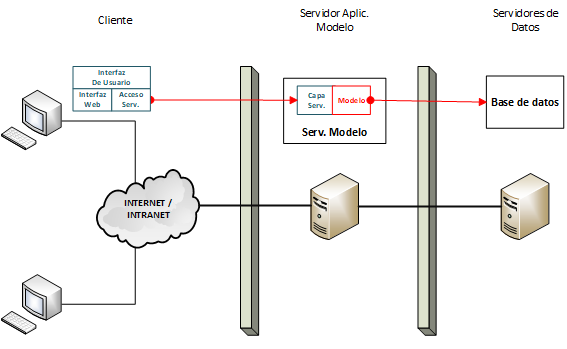
\includegraphics[
   keepaspectratio=true
]{./05_Diseno/arq3capas.png}
\caption{Diagrama arquitectura en tres capas}
\end{figure}

\begin{itemize} [label={}]
	\item \textbf{Capa Servidor de Datos: } Es la capa encargada de gestionar el almacenamiento de los datos.
	\item \textbf{Capa Servidor Aplicación:} Formada por la capa de  servicios y el modelo. La capa de servicios, sirve de enlace entre la interfaz de usuario y el modelo mientras que el modelo, comúnmente, se subdivide en dos: la subcapa de acceso a datos y la subcapa de lógica de negocio.
	En la primera de ellas, se lleva acabo todas las acciones relacionadas con el acceso a los datos y es la que mantiene la comunicación con el servidor de datos.
	Por su parte, la subcapa de lógica de negocio, se encarga de llevar a cabo la implementación de las funcionalidades de la aplicación.
	\item \textbf{Capa Interfaz de Usuario: } Corresponde con la interfaz gráfica que se instala en las máquinas clientes y dispositivos finales. 
\end{itemize}



\subsection{Arquitectura en 4 capas}
En esta alternativa, se añade una capa intermedia entre el cliente y el modelo que actúe de servidor de aplicaciones y que proporciones la interfaz web para clientes que accedan desde navegador web.

\begin{figure}[!h]

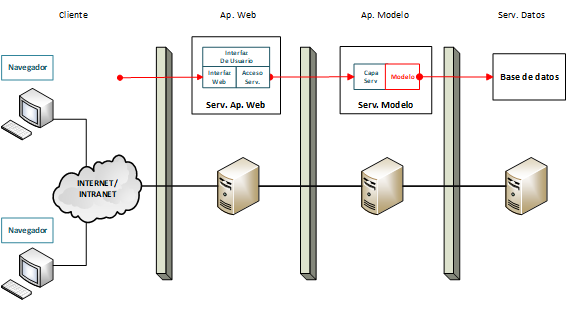
\includegraphics[
   keepaspectratio=true
]{./05_Diseno/arq4capas.png}
\caption{Diagrama arquitectura en cuatro capas}
\end{figure}

Un navegador, para acceder a la aplicación, necesitará de un servidor de aplicaciones que le proporciones la interfaz web. Incorporar esta interfaz dentro del servidor de aplicaciones visto en la arquitectura anterior haría que este y el modelo estén fuertemente acoplados, impidiendo que puedan ser construidos con tecnologías diferentes.

Por ello, con esta arquitectura se pretende hacer ese desacople consiguiendo que múltiples aplicaciones pueden invocar al modelo, independientemente de que sean con interfaz gráfica o mediante navegador, sin necesidad de replicar el código del modelo en cada aplicación.

En consecuente, analizados los requisitos del sistema y conociendo las necesidades del mismo, se diseñará un sistema basado en una arquitectura de cuatro capas.


\subsection{Arquitectura completa del sistema}
A continuación, se presenta el diseño completo que se elaborará en la aplicación.

\begin{figure}[!h]

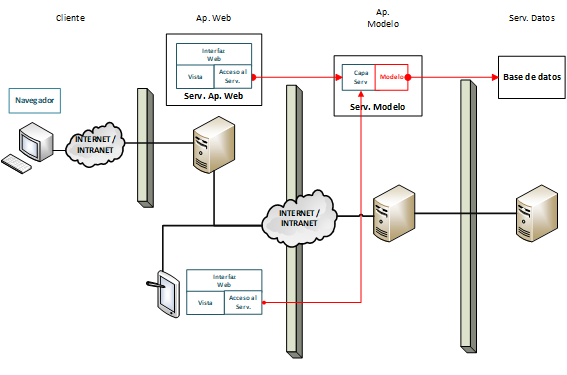
\includegraphics[
   keepaspectratio=true
]{./05_Diseno/arqsistema.png}
\caption{Diagrama arquitectura completa del sistema}
\end{figure}

Como se puede observar en el diagrama, el sistema sigue una arquitectura en cuatro capas.

Al tener la aplicación modelo desacoplada de la aplicación web, la capa de servicios debe servir de enlace entre la capa modelo y la interfaz de usuario. Ese enlace lo ofrece mediante unos servicios REST, que exponen a la capa superior, las funcionalidades implementadas en la capa modelo.

Por su parte, las aplicaciones cliente, tanto la interfaz de usuario del cliente móvil como la interfaz web del servidor de aplicaciones, siguen el patrón de arquitectura Modelo-Vista-Controlador (MVC). En ellas, el modelo no se encuentra implementado en la propia aplicación, sino que es accedido mediante un cliente REST que consume los servicios ofrecidos por la capa de servicios del modelo. De esta forma, ambas aplicaciones finales, invocan al modelo sin necesidad de tenerlo replicado.


\section{Capa Modelo}
Esta capa es la encargada de implementar la lógica de negocio de la aplicación, lo que implica el manejo de las entidades persistentes y el acceso a los datos. Como podemos observar en la Figura 6.4, y debido a la arquitectura establecida, el modelo estará compuesto por una subcapa de acceso a datos, otra de lógica de negocio y una última de servicios REST, la que permitirá acceder remotamente a las funcionalidades de la aplicación independientemente del tipo de  cliente final.

\begin{figure}[H]
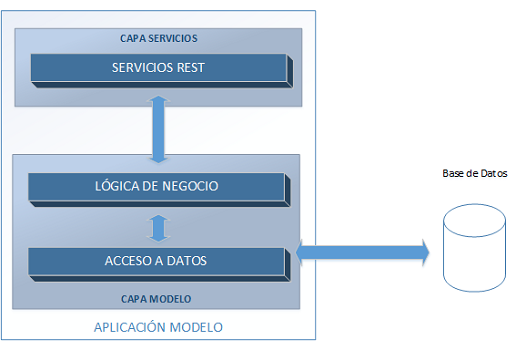
\includegraphics[
   keepaspectratio=true
]{./05_Diseno/disenomodelo.png}
\caption{Diagrama diseño modelo}
\end{figure}


\newpage
\subsection{Diagrama clases persistentes}
\begin{figure}[H]
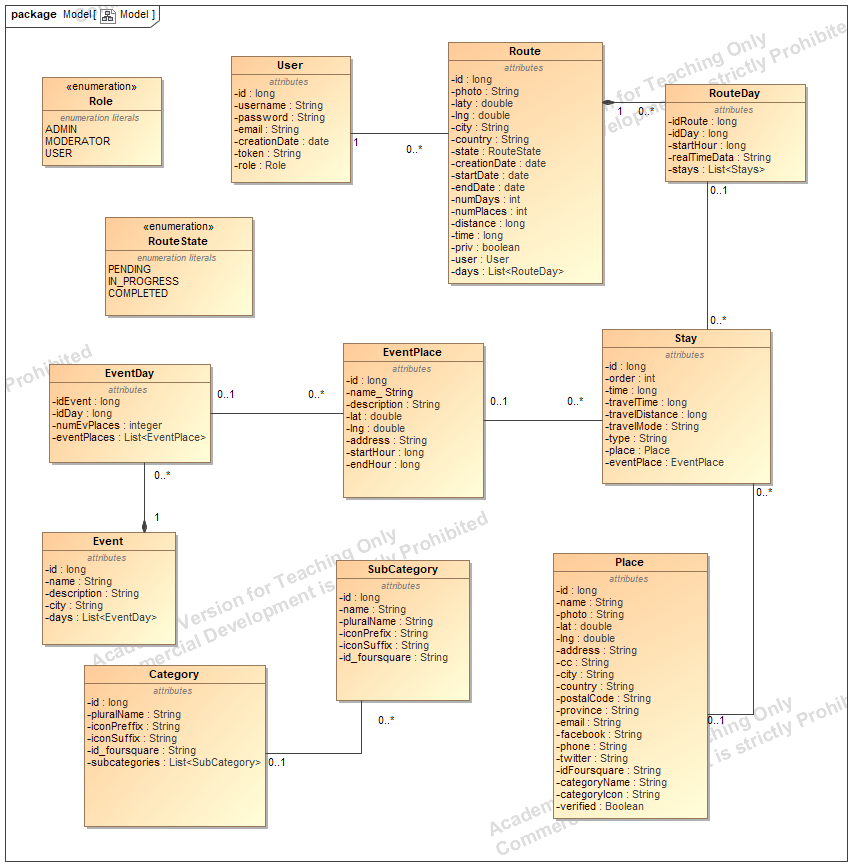
\includegraphics[
   keepaspectratio=true
]{./05_Diseno/disenoclases.png}
\caption{Diagrama diseño modelo}
\end{figure}

En el diagrama se muestran las clases persistentes que manejará la aplicación. A continuación, se detallará brevemente, el significado y funcionalidad de cada una:

\begin{itemize}
	\item \textbf{User: } Es la clase encargada de gestionar la información de los usuarios registrados en la aplicación.
	\item \textbf{Role: } Enumerado con los roles disponibles para un usuario: \textit{ADMIN, MODERATOR y USER}.
	\item \textbf{Route: } Clase encargada de guardar la información sobre las rutas creadas por los usuarios. Las rutas están compuestas por \textit{RouteDays}.
	\item \textbf{RouteDay: } Clase con una relación fuerte de composición con la clase \textit{Route}. Su tiempo de vida está condicionada por la vida de la clase que la incluye. Mantiene la información para cada uno de los días que componen la duración de una ruta.
	\item \textbf{RouteState: } Enumerado con los diferentes estados por los que pasa una ruta en el tiempo: \textit{PENDING, IN\_PROGRESS y COMPLETED}.
	\item \textbf{Stay: } Entidad con la funcionalidad de gestionar las visitas que decida hacer un usuario en un día de una ruta determinada. La visita, puede ser a lugares obtenidos de una fuente externa (\textit{Foursquare}) o a eventos gestionados por la propia aplicación.
	\item \textbf{Place: } Entidad que registra y almacena los detalles sobre los lugares extraídos de la fuente externa.
	\item \textbf{Event: } Es la clase encargada de gestionar los eventos dados de alto en el sistema. Los eventos están compuestos por \textit{EventDays}.
	\item \textbf{EventDay: } Clase con una relación fuerte de composición con la clase \textit{Event}. Su tiempo de vida está condicionada por la vida de la clase que la incluye. Mantiene la información para cada uno de los días que componen al evento.
	\item \textbf{EventPlace: } Es la clase donde se maneja toda la información sobre las distintas ubicaciones y actividades que incluye un día determinado del evento.
	\item \textbf{Category: } Clase que almacena la información relevante a las categorías sobre las que se filtran los lugares obtenidos de \textit{Foursquare}.
	\item \textbf{SubCategory: } Establece una jerarquía con la clase anterior. Almacena las categorías que son un subtipo de una categoría determinada.
\end{itemize}

\subsection{Diseño módulo acceso a datos}
En esta capa se hará uso del patrón de diseño Data-Access-Object (DAO).

\subsubsection*{Patrón de diseño DAO}
Este patrón de diseño intenta desacoplar el acceso a los datos de su almacenamiento subyacente. Los datos persistentes, actualmente, dependen en gran medida del tipo de base de datos utilizada: base de datos relacional, base de datos orientada a objetos, archivos planos... siendo las bases de datos relacionales las más utilizadas. Lamentablemente, se acceden a estes tipos de bases de datos de maneras muy diferentes y sería preferible elegir el tipo de base de datos utilizada en la fase de implementación en lugar de en la fase de diseño.

Utilizar este patrón en lugar de acceder directamente a la fuente de datos nos permite pasar de un tipo de fuente de datos a otro diferente sin tener que realizar modificaciones en la lógica.


\begin{figure}[H]
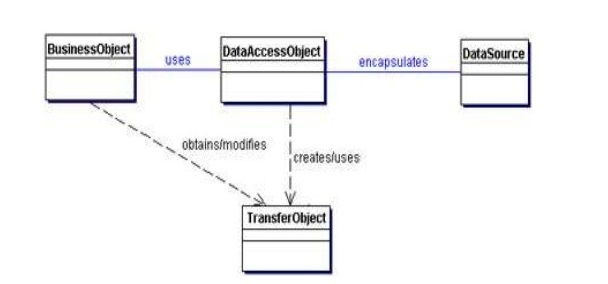
\includegraphics[
   keepaspectratio=true
]{./05_Diseno/patrondao.jpg}
\caption{Diagrama diseño modelo}
\end{figure}

En la Figura 6.6 se muestra un pequeño diagrama con los elementos participantes en este patrón de diseño.

\begin{itemize}
	\item \textbf{Business Object: } Representa la clase con la lógica de negocio. Es la responsable de saber qué y cómo modificar el contenido de los datos pero no como almacenarlo.
	\item \textbf{Data Access Object: } Se encarga de ocultar la fuente de datos real de manera que el objeto con la lógica de negocio (Business Object) se comunica con este en vez de hacerlo directamente con el objeto de acceso a los datos.
	\item \textbf{DataSource: } Es la fuente real de datos y el que realiza la conexión con la base de datos. En la mayoría de casos, existe una base de datos relacional a la que se accede a través de SQL.
	\item \textbf{Transfer Object: } Es el objeto que se utiliza para transferir el contenido de los datos reales del \textit{Data Access Object} al objeto de negocio \textit{Business Object}. Representa los datos almacenados en la base de datos.
\end{itemize}

\subsection{Diseño módulo lógica de negocio}
\subsection{Diseño módulo servicios REST}
\section{Controlador}
\subsection{Aplicación web}
\subsection{Aplicación móvil}

\section{Diseño físco de los datos}
\subsection{Modelo Entidad-Relación}
\subsection{Modelo Relacional}






